\section{Solver  Class Reference}
\label{classSolver}\index{Solver@{Solver}}
The base class for all path planners. 


{\tt \#include $<$solver.h$>$}

Inheritance diagram for Solver::\begin{figure}[H]
\begin{center}
\leavevmode
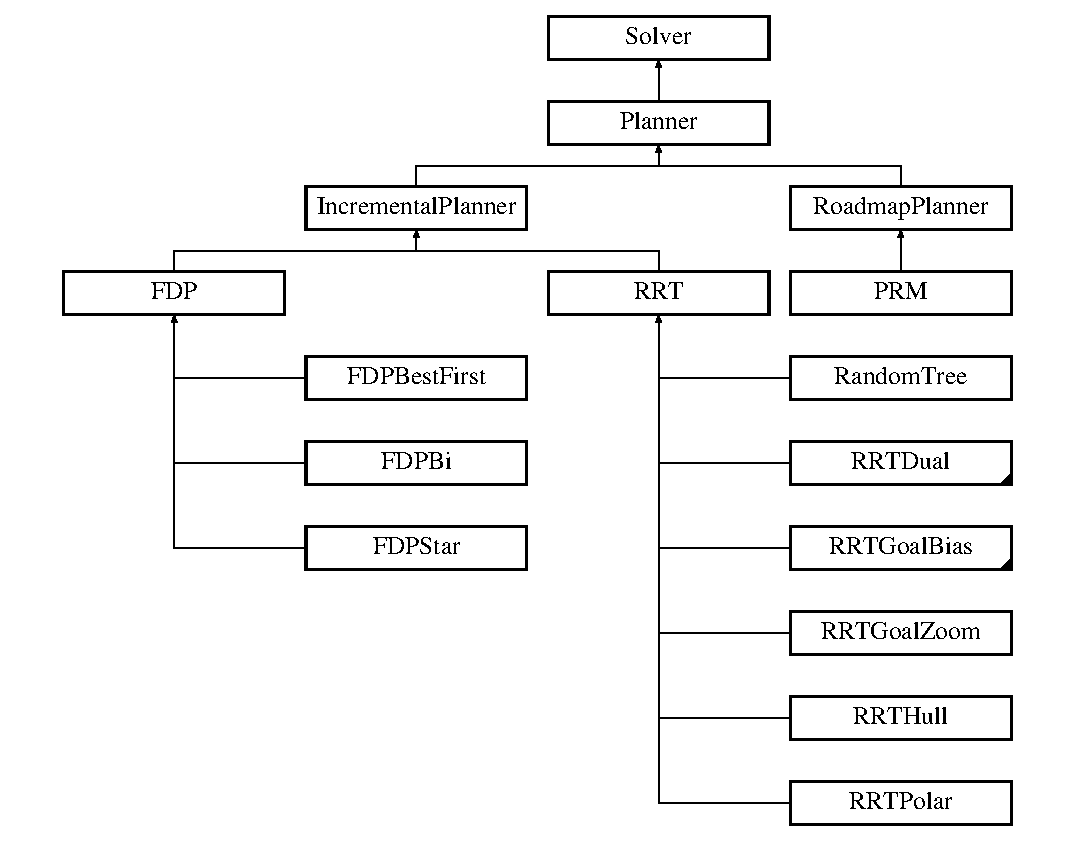
\includegraphics[height=10cm]{classSolver}
\end{center}
\end{figure}
\subsection*{Public Methods}
\begin{CompactItemize}
\item 
{\bf Solver} ({\bf Problem} $\ast$problem)
\begin{CompactList}\small\item\em A constructor that initializes data members.\item\end{CompactList}\item 
virtual {\bf $\sim$Solver} ()
\begin{CompactList}\small\item\em Empty destructor.\item\end{CompactList}\end{CompactItemize}
\subsection*{Public Attributes}
\begin{CompactItemize}
\item 
string {\bf File\-Path}
\begin{CompactList}\small\item\em The directory in which all files for a problem will be stored.\item\end{CompactList}\item 
{\bf Problem}$\ast$ {\bf P}
\begin{CompactList}\small\item\em An instance of problem, which defines all of the problem-specific methods needed for solvers.\item\end{CompactList}\end{CompactItemize}


\subsection{Detailed Description}
The base class for all path planners.



\subsection{Constructor \& Destructor Documentation}
\index{Solver@{Solver}!Solver@{Solver}}
\index{Solver@{Solver}!Solver@{Solver}}
\subsubsection{\setlength{\rightskip}{0pt plus 5cm}Solver::Solver ({\bf Problem} $\ast$ {\em problem})}\label{classSolver_a0}


A constructor that initializes data members.

\index{Solver@{Solver}!~Solver@{$\sim$Solver}}
\index{~Solver@{$\sim$Solver}!Solver@{Solver}}
\subsubsection{\setlength{\rightskip}{0pt plus 5cm}Solver::$\sim$Solver ()\hspace{0.3cm}{\tt  [inline, virtual]}}\label{classSolver_a1}


Empty destructor.



\subsection{Member Data Documentation}
\index{Solver@{Solver}!FilePath@{FilePath}}
\index{FilePath@{FilePath}!Solver@{Solver}}
\subsubsection{\setlength{\rightskip}{0pt plus 5cm}string Solver::File\-Path}\label{classSolver_m0}


The directory in which all files for a problem will be stored.

\index{Solver@{Solver}!P@{P}}
\index{P@{P}!Solver@{Solver}}
\subsubsection{\setlength{\rightskip}{0pt plus 5cm}{\bf Problem} $\ast$ Solver::P}\label{classSolver_m1}


An instance of problem, which defines all of the problem-specific methods needed for solvers.

This includes incremental simulation and collision detection. 

The documentation for this class was generated from the following files:\begin{CompactItemize}
\item 
{\bf solver.h}\item 
{\bf solver.C}\end{CompactItemize}
